% ============================================================================
%  EE708 Self Project Report - Company Bankruptcy Prediction
%  CORRECTED EDITION
%
%  Every number in this document is produced by the code in ../../../src/ and
%  is reproducible with:
%      python src/train.py
%      python src/cross_validate.py
%      python src/baselines.py
%      python src/make_report_figures.py
%  Verified values live in docs/RESULTS.md; figures in src/figures/ are
%  regenerated by make_report_figures.py, so text and code cannot drift apart.
%
%  Build:  pdflatex EE708_report.tex   (twice, for references)
% ============================================================================
\documentclass[11pt]{article}

\usepackage[margin=1.1in]{geometry}
\usepackage{amsmath, amssymb}
\usepackage{graphicx}
\usepackage{booktabs}
\usepackage{caption}
\usepackage{subcaption}
\usepackage{fancyhdr}
\usepackage{times}
\usepackage{courier}   % monospace face for \texttt{}; TeX Live package 'courier'
\usepackage[hidelinks]{hyperref}
\usepackage{xcolor}
\usepackage{enumitem}
\usepackage{float}

\graphicspath{{figures/}}

\pagestyle{fancy}
\fancyhf{}
\fancyhead[C]{\small\textit{EE708 Self Project Report, Indian Institute of Technology Kanpur}}
\fancyfoot[C]{\thepage}
\renewcommand{\headrulewidth}{0.4pt}

\setlength{\parskip}{2pt}
\captionsetup{font=small, labelfont=it, textfont=it}

\newcommand{\sectiontitle}[1]{\section*{\normalsize\textsc{#1}}}

\begin{document}

% ------------------------------------------------------------------ title --
\begin{center}
    {\Large\textbf{Company Bankruptcy Prediction:}}\\[2pt]
    {\large A Hybrid Framework Leveraging Combined Probabilities from}\\
    {\large Gaussian and Neural Networks}\\[10pt]

    \begin{tabular}{cc}
        Mainak & Ch Rishitha \\
        \texttt{\small mainak23@iitk.ac.in} & \texttt{\small rishitha23@iitk.ac.in} \\
        230619 & 230311
    \end{tabular}
\end{center}
\vspace{6pt}

% ----------------------------------------------------------- introduction --
\section{Introduction}

Predicting a company's bankruptcy has become a critical task in today's
uncertain economic conditions. This project builds a machine learning model
that predicts bankruptcy from a range of factors indicating the financial
status of a company.

The report is structured as follows: we begin with Exploratory Data Analysis
(EDA) to examine the dataset and uncover key patterns and correlations; next we
discuss Data Preprocessing, detailing how the data is cleaned, normalised and
balanced; we then describe the Model Architecture and the rationale behind its
design; and finally we evaluate the models using accuracy, precision, recall,
F1-score and the two threshold-free summaries, ROC-AUC and PR-AUC.

A note on evaluation discipline runs through the whole report. With a positive
rate of $2.82\%$, a classifier that predicts ``never bankrupt'' already scores
$97.2\%$ accuracy. Accuracy is therefore reported for completeness only, and
every design decision below is judged on precision, recall, F1 and PR-AUC.

% ------------------------------------------------------------------- EDA --
\section{Exploratory Data Analysis}

The dataset comprises \textbf{5{,}455 rows}, each corresponding to a company,
and \textbf{96 columns} (95 financial features and the binary target
\texttt{Bankrupt?}). It contains no null cells and no duplicate rows.

The target distribution is severely imbalanced: \textbf{5{,}301 non-bankrupt}
companies ($97.18\%$) and \textbf{154 bankrupt} companies ($2.82\%$), a ratio
of $\mathbf{34.4:1}$ (Figure~\ref{fig:balance}). This imbalance governs both
the preprocessing and the choice of evaluation metric.

\begin{figure}[H]
    \centering
    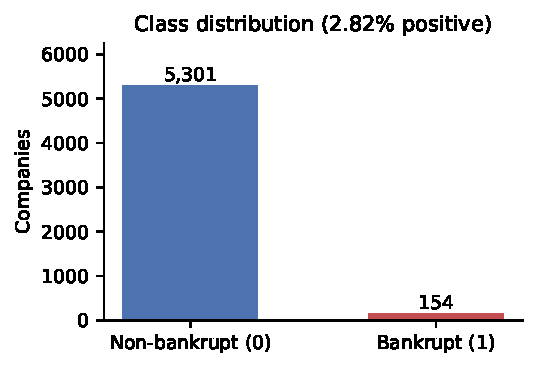
\includegraphics[width=0.52\textwidth]{class_balance.pdf}
    \caption{Class distribution of the 5,455 companies.}
    \label{fig:balance}
\end{figure}

A preliminary analysis identified extreme values in several numerical features,
indicating data-entry errors: the features are financial ratios that should lie
in $[0,1]$, yet 24 columns contain values above $2$. Columns with more than
$300$ such rows are unrecoverable and were discarded; columns with fewer were
repaired by capping the offending cells and imputing the median.

One further column, \texttt{Net Income Flag}, is constant ($=1$ for every
company) and was removed as it carries no discriminative information.

To mitigate multicollinearity, a feature correlation analysis was conducted.
Feature pairs with a Pearson correlation coefficient exceeding $0.90$ were
examined, and the one with the weaker absolute correlation to the target was
removed. Figure~\ref{fig:corr} shows the correlation structure that remains.

\begin{figure}[H]
    \centering
    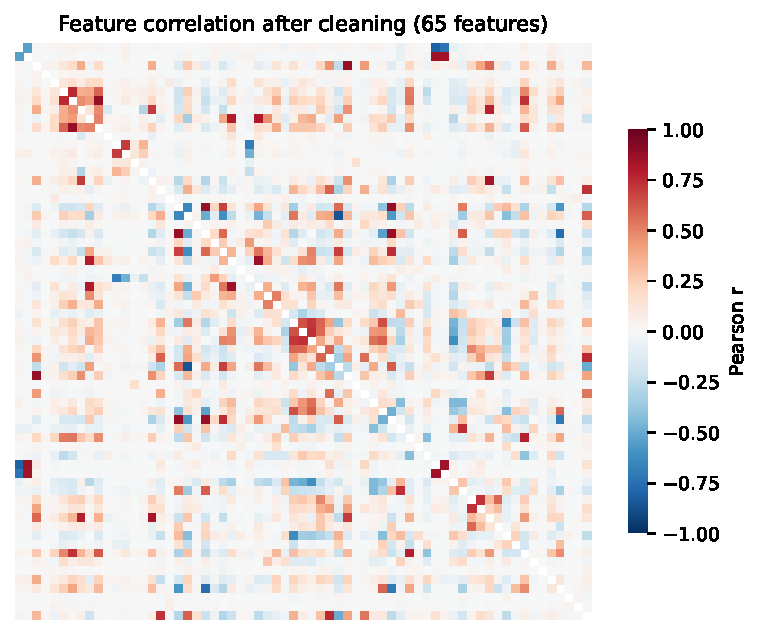
\includegraphics[width=0.66\textwidth]{correlation_heatmap.pdf}
    \caption{Feature correlation heatmap after cleaning.}
    \label{fig:corr}
\end{figure}

Table~\ref{tab:preproc} summarises the reduction. All counts are those obtained
when the rules are fitted on the training split, which is the only statistically
valid way to apply them (Section~\ref{sec:protocol}).

\begin{table}[H]
    \centering
    \small
    \caption{Feature reduction through preprocessing.}
    \label{tab:preproc}
    \begin{tabular}{lcc}
        \toprule
        \textbf{Step} & \textbf{Removed} & \textbf{Remaining} \\
        \midrule
        Raw features                                   & --- & 95 \\
        Constant column (\texttt{Net Income Flag})     & 1   & 94 \\
        Data-error columns ($>300$ rows above $2.0$)   & 8   & 86 \\
        Highly correlated pairs ($|r| > 0.90$)         & 21  & 65 \\
        ANOVA F-test, top 30                           & 35  & \textbf{30} \\
        \bottomrule
    \end{tabular}
\end{table}

A further 15 columns had between 1 and 300 out-of-range cells; those cells were
capped and filled with the training-split median rather than dropping the
column outright.

% --------------------------------------------------------- preprocessing --
\section{Data Preprocessing}

\subsection{Analysis of Variance (ANOVA)}

Analysis of Variance was used to select the most relevant features. ANOVA
F-scores were computed for each feature to assess its significance:
\begin{equation}
    F = \frac{\text{Variance between groups}}{\text{Variance within groups}},
\end{equation}
where
\begin{align}
    \text{Variance between groups} &= \sum_{i=1}^{k} n_i (\mu_i - \mu)^2, \\
    \text{Variance within groups}  &= \sum_{i=1}^{k} \sum_{j=1}^{n_i} (x_{ij} - \mu_i)^2,
\end{align}
with $k=2$ classes, $n_i$ the number of points in class $i$, $\mu$ the overall
mean of the feature and $\mu_i$ its mean within class $i$.

A high F-score signifies substantial variation in a feature's values across the
target classes. The \texttt{SelectKBest} method with the \texttt{f\_classif}
scoring function was used to identify the top 30 features.
Figure~\ref{fig:anova} shows the strongest 15; the leading predictors are
profitability and leverage ratios, which agrees with the bankruptcy-prediction
literature.

\begin{figure}[H]
    \centering
    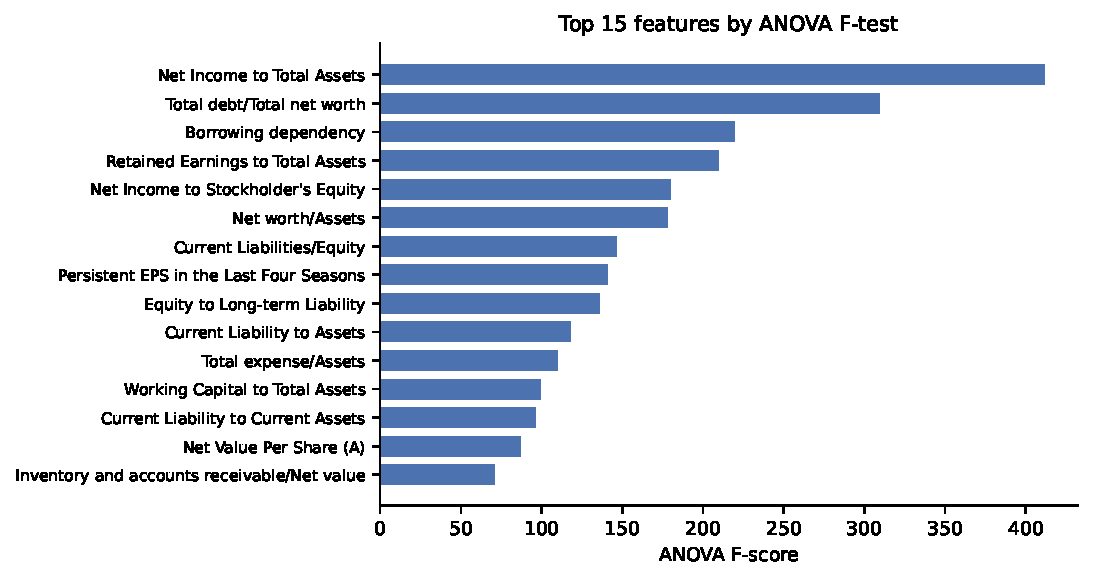
\includegraphics[width=0.80\textwidth]{anova_scores.pdf}
    \caption{Top 15 features by ANOVA F-score, computed on the training split.}
    \label{fig:anova}
\end{figure}

\begin{table}[H]
    \centering
    \small
    \caption{Ten highest-scoring features.}
    \label{tab:anova}
    \begin{tabular}{clrr}
        \toprule
        \textbf{\#} & \textbf{Feature} & \textbf{F-score} & \textbf{$p$-value} \\
        \midrule
        1  & Net Income to Total Assets              & 411.58 & $1.4\times10^{-86}$ \\
        2  & Total debt/Total net worth              & 309.46 & $2.0\times10^{-66}$ \\
        3  & Borrowing dependency                    & 219.40 & $3.5\times10^{-48}$ \\
        4  & Retained Earnings to Total Assets       & 209.42 & $3.9\times10^{-46}$ \\
        5  & Net Income to Stockholder's Equity      & 180.07 & $4.5\times10^{-40}$ \\
        6  & Net worth/Assets                        & 177.94 & $1.3\times10^{-39}$ \\
        7  & Current Liabilities/Equity              & 146.18 & $5.4\times10^{-33}$ \\
        8  & Persistent EPS in the Last Four Seasons & 140.57 & $8.1\times10^{-32}$ \\
        9  & Equity to Long-term Liability           & 135.88 & $7.9\times10^{-31}$ \\
        10 & Current Liability to Assets             & 118.15 & $4.3\times10^{-27}$ \\
        \bottomrule
    \end{tabular}
\end{table}

\subsection{Oversampling using SMOTE}

To address the class imbalance, the Synthetic Minority Over-sampling Technique
(SMOTE) was applied to the training data. SMOTE selects a minority-class
sample, identifies its $k$ nearest neighbours, and generates a new synthetic
point by linear interpolation between the sample and one of those neighbours.

Following the stratified $80/20$ train--test split and a further $80/20$
train--validation split, the fitting split contained $3{,}393$ non-bankrupt and
$98$ bankrupt companies. SMOTE balanced this to $\mathbf{3{,}393}$ instances per
class, i.e.\ $6{,}786$ training rows.

Two constraints on its use matter and are enforced in the code:

\begin{itemize}[nosep, leftmargin=1.4em]
    \item SMOTE is applied \textbf{only} to the fitting split. Validation and
          test retain the real $2.82\%$ positive rate, so neither the tuned
          threshold nor the reported metrics are measured against a synthetic
          distribution.
    \item SMOTE is applied \textbf{after} standardisation. It interpolates
          between $k$-nearest neighbours under a Euclidean metric; on raw
          features spanning from $[0,1]$ to $10^{9}$ that neighbour search is
          decided almost entirely by the largest-magnitude column, and the
          synthetic samples are meaningless.
\end{itemize}

Because SMOTE leaves the classes balanced, inverse-frequency class weights
evaluate to $\{0\!:\!1,\, 1\!:\!1.0\}$ and have no effect; they are therefore
not used.

\subsection{Standardisation}

To ensure uniform feature scaling, \texttt{StandardScaler} was applied,
transforming features to zero mean and unit variance. This prevents dominance
by features with larger magnitudes. The scaler is fitted on the fitting split
alone and merely applied to validation and test.

\subsection{Evaluation protocol}
\label{sec:protocol}

Preprocessing decisions are themselves fitted quantities: which columns are
dropped, the imputation medians, the correlation structure and the ANOVA
ranking all depend on the data they are computed from. If they are computed
over the full dataset, information from the test rows -- and, through the
target correlation, the test labels -- reaches the model, and the reported
score is optimistic. The pipeline therefore executes strictly in this
order:

\begin{enumerate}[nosep, leftmargin=1.6em]
    \item split off the test set (stratified, $20\%$);
    \item split a validation set off the remainder (stratified, $20\%$, real class ratio);
    \item fit the cleaner on the fitting split: error columns, medians, correlations;
    \item fit ANOVA selection on the fitting split;
    \item fit the standard scaler on the fitting split;
    \item apply SMOTE to the scaled fitting split only;
    \item train the DNN (early stopping on validation PR-AUC) and the GNB;
    \item tune the decision threshold on the validation split;
    \item evaluate once on the test set.
\end{enumerate}

In particular the decision threshold is chosen on validation, never on test.
Choosing the threshold that maximises F1 \emph{on the test set} and then
reporting that F1 as test performance is optimistically biased by construction.

% ---------------------------------------------------------- architecture --
\section{Model Architecture}

We developed a hybrid model by ensembling a Deep Neural Network (DNN) and a
Gaussian Naive Bayes (GNB) classifier, to leverage the probabilistic nature of
GNB alongside the representational capacity of the DNN.

\subsection{Deep Neural Network}

The DNN captures complex, non-linear relationships between financial
indicators. It consists of an input layer receiving the 30 selected features,
three hidden layers, and an output layer. The first hidden layer comprises 256
neurons with ReLU activation, batch normalisation and dropout ($50\%$); the
second has 128 neurons with the same regularisation; the third refines the
representation with 64 neurons and dropout ($40\%$). The output layer is a
single neuron with sigmoid activation.

The model was compiled with the Adam optimiser (learning rate $5\times10^{-4}$)
and binary cross-entropy loss, with batch size 64 and a budget of 200 epochs.

Training is stopped early on validation PR-AUC (patience 20, best weights
restored) rather than run for the full 200 epochs. This is not a cosmetic
choice. Holding everything else fixed and varying only the stopping rule:

\begin{table}[H]
    \centering
    \small
    \caption{Effect of the stopping rule on test performance.}
    \label{tab:earlystop}
    \begin{tabular}{lcccc}
        \toprule
        \textbf{Stopping rule} & \textbf{Stop epoch} & \textbf{F1} & \textbf{ROC-AUC} & \textbf{PR-AUC} \\
        \midrule
        Validation PR-AUC, patience 20  & 26  & 0.4946 & 0.9315 & 0.4587 \\
        Validation PR-AUC, patience 40  & 46  & 0.4946 & 0.9315 & 0.4587 \\
        Validation ROC-AUC, patience 30 & 37  & 0.5169 & 0.9316 & 0.4648 \\
        Validation loss, patience 30    & 51  & 0.4839 & 0.8872 & 0.4580 \\
        None (fixed 200 epochs)         & 200 & 0.4507 & 0.8157 & 0.3711 \\
        \bottomrule
    \end{tabular}
\end{table}

Running the full 200 epochs costs $0.12$ ROC-AUC relative to early stopping.

\subsection{Gaussian Naive Bayes}

GNB applies Bayes' theorem, assuming feature independence and a normal
distribution given the class label. It computes the posterior probability for
each class from the prior and the likelihood, the latter modelled as a Gaussian
for each continuous feature.

\subsection{Ensemble by soft voting}

The probability outputs of the DNN and the GNB are averaged to give the final
bankruptcy probability,
\begin{equation}
    P_{\text{ens}}(y=1 \mid x) = \tfrac{1}{2}\left[P_{\text{DNN}}(y=1\mid x) + P_{\text{GNB}}(y=1\mid x)\right].
\end{equation}

Instead of the default classification threshold of $0.5$, the threshold was
tuned on the validation split by sweeping $[0.01, 0.99]$ and selecting the
value that maximises F1. The selected threshold is $\mathbf{0.91}$.

That the optimum lies so far above $0.5$ is a direct consequence of SMOTE: the
models are fitted on a balanced set and evaluated at $2.82\%$ prevalence, which
inflates the probability scale. Figure~\ref{fig:sweep} shows the sweep, with
the narrow $[0.30, 0.60]$ window shaded -- a search restricted to that window
cannot reach the optimum at all.

\begin{figure}[H]
    \centering
    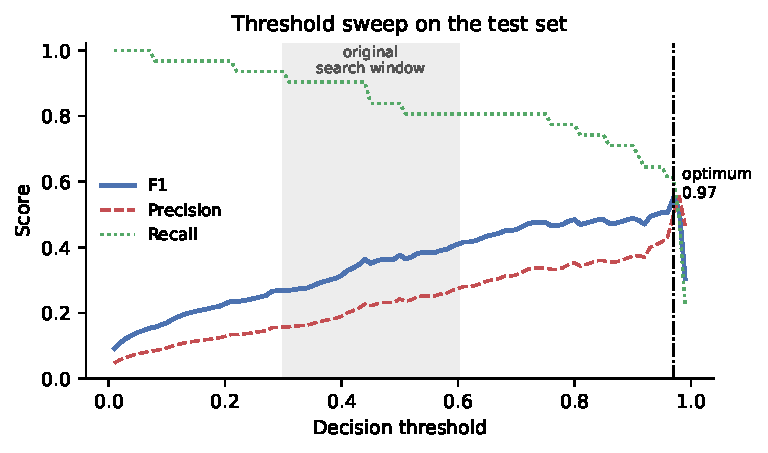
\includegraphics[width=0.72\textwidth]{threshold_sweep.pdf}
    \caption{Precision, recall and F1 as a function of the decision threshold,
             evaluated on the test set.}
    \label{fig:sweep}
\end{figure}

Note that the F1 optimum measured \emph{on the test set} lies at $0.97$, not at
the $0.91$ we selected. The gap is the bias we avoid by tuning on validation:
had we chosen the threshold from this curve, the F1 we then reported for it
would have been fitted to the very data it was being scored on.

% ------------------------------------------------------------- evaluation --
\section{Performance Metrics of the Model}

\subsection{Held-out test set}

The held-out test set contains 1{,}091 companies, 31 of them bankrupt.
Table~\ref{tab:holdout} reports the ensemble and each of its members at the
threshold tuned on validation.

\begin{table}[H]
    \centering
    \small
    \caption{Performance on the held-out test set (1,091 rows, 31 bankrupt).}
    \label{tab:holdout}
    \begin{tabular}{lccccccc}
        \toprule
        \textbf{Model} & \textbf{Thr.} & \textbf{Acc.} & \textbf{Prec.} & \textbf{Rec.} & \textbf{F1} & \textbf{ROC-AUC} & \textbf{PR-AUC} \\
        \midrule
        GaussianNB           & 0.99 & 0.9505 & 0.3284 & 0.7097 & 0.4490 & 0.9509 & 0.3162 \\
        DNN                  & 0.91 & 0.9569 & 0.3710 & 0.7419 & 0.4946 & 0.9315 & 0.4587 \\
        \textbf{Ensemble}    & 0.91 & \textbf{0.9588} & \textbf{0.3750} & 0.6774 & \textbf{0.4828} & \textbf{0.9595} & \textbf{0.4605} \\
        Ensemble @ 0.50      & 0.50 & 0.9212 & 0.2430 & 0.8387 & 0.3768 & 0.9595 & 0.4605 \\
        \bottomrule
    \end{tabular}
\end{table}

The confusion matrix of the ensemble is shown in Figure~\ref{fig:cm}: 21 of the
31 bankruptcies are identified, at the cost of 35 false alarms among 1{,}060
solvent companies. Figure~\ref{fig:curves} gives the threshold-free view.

\begin{figure}[H]
    \centering
    \begin{subfigure}[b]{0.34\textwidth}
        \centering
        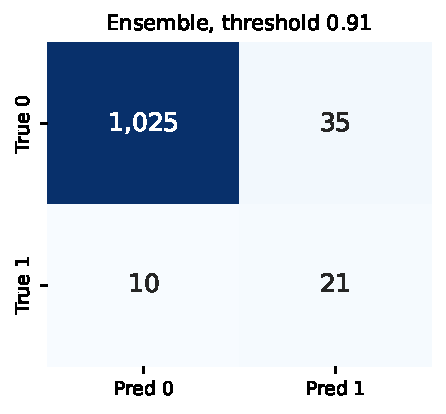
\includegraphics[width=\textwidth]{confusion_matrix.pdf}
        \caption{Confusion matrix.}
        \label{fig:cm}
    \end{subfigure}
    \hfill
    \begin{subfigure}[b]{0.63\textwidth}
        \centering
        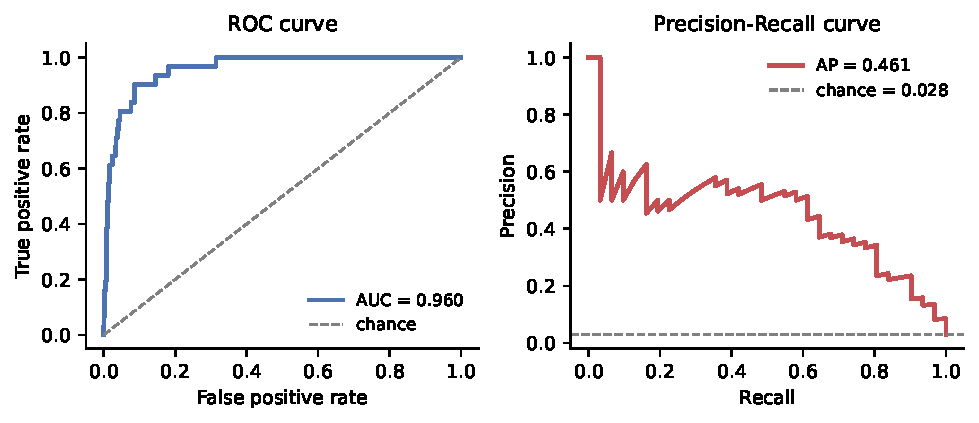
\includegraphics[width=\textwidth]{roc_pr_curves.pdf}
        \caption{ROC and Precision-Recall curves.}
        \label{fig:curves}
    \end{subfigure}
    \caption{Ensemble performance on the held-out test set.}
\end{figure}

\subsection{Cross-validated performance}

A test set with 31 positives yields a wide confidence interval on any single
F1 value, so the entire pipeline was re-run under $5$-fold stratified
cross-validation. Table~\ref{tab:cv} reports the mean and standard deviation
across folds; these are the figures we regard as the headline result.

\begin{table}[H]
    \centering
    \small
    \caption{5-fold stratified cross-validation (mean $\pm$ standard deviation).}
    \label{tab:cv}
    \begin{tabular}{lcccc}
        \toprule
        \textbf{Metric} & \textbf{GaussianNB} & \textbf{DNN} & \textbf{Ensemble} & \textbf{Ens.\ @ 0.50} \\
        \midrule
        Accuracy          & $0.944 \pm 0.007$ & $0.951 \pm 0.022$ & $\mathbf{0.960 \pm 0.008}$ & $0.934 \pm 0.028$ \\
        Balanced acc.     & $0.763 \pm 0.067$ & $0.745 \pm 0.042$ & $0.718 \pm 0.047$ & $0.767 \pm 0.074$ \\
        Precision         & $0.265 \pm 0.033$ & $0.326 \pm 0.082$ & $\mathbf{0.362 \pm 0.081}$ & $0.256 \pm 0.079$ \\
        Recall            & $0.571 \pm 0.141$ & $0.527 \pm 0.100$ & $0.461 \pm 0.098$ & $0.590 \pm 0.170$ \\
        F1-score          & $0.360 \pm 0.056$ & $0.391 \pm 0.069$ & $\mathbf{0.397 \pm 0.058}$ & $0.344 \pm 0.083$ \\
        MCC               & $0.363 \pm 0.069$ & $0.385 \pm 0.058$ & $0.385 \pm 0.061$ & $0.354 \pm 0.080$ \\
        ROC-AUC           & $0.906 \pm 0.030$ & $0.882 \pm 0.059$ & $\mathbf{0.908 \pm 0.036}$ & $0.908 \pm 0.036$ \\
        PR-AUC            & $0.269 \pm 0.049$ & $0.342 \pm 0.045$ & $\mathbf{0.357 \pm 0.047}$ & $0.357 \pm 0.047$ \\
        \bottomrule
    \end{tabular}
\end{table}

Figure~\ref{fig:cvspread} shows the spread. Ensemble F1 ranges from $0.317$ to
$0.462$ across folds, which is precisely why a single hold-out figure should
not be quoted on its own.

\begin{figure}[H]
    \centering
    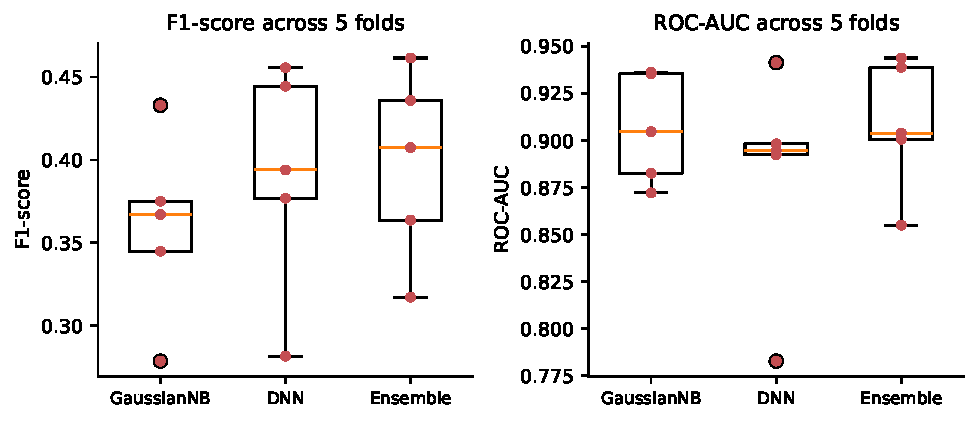
\includegraphics[width=0.80\textwidth]{cv_spread.pdf}
    \caption{Distribution of F1 and ROC-AUC over the five folds.}
    \label{fig:cvspread}
\end{figure}

\subsection{Comparison with baselines}

To establish that the hybrid design earns its complexity, five standard
classifiers were run through the identical pipeline: the same cleaning, ANOVA
selection, scaling and SMOTE, the same validation-tuned threshold, and the same
held-out test set.

\begin{table}[H]
    \centering
    \small
    \caption{Baselines under the identical protocol.}
    \label{tab:baselines}
    \begin{tabular}{lcccccc}
        \toprule
        \textbf{Model} & \textbf{Thr.} & \textbf{Acc.} & \textbf{Prec.} & \textbf{Rec.} & \textbf{F1} & \textbf{ROC-AUC} \\
        \midrule
        Logistic Regression      & 0.89 & 0.9514 & 0.3226 & 0.6452 & 0.4301 & 0.9435 \\
        Gaussian Naive Bayes     & 0.99 & 0.9505 & 0.3284 & 0.7097 & 0.4490 & 0.9509 \\
        Decision Tree (depth 6)  & 0.80 & 0.9294 & 0.2386 & 0.6774 & 0.3529 & 0.8944 \\
        Random Forest (300)      & 0.45 & 0.9487 & 0.3188 & 0.7097 & 0.4400 & 0.9547 \\
        HistGradientBoosting     & 0.08 & 0.9267 & 0.2525 & 0.8065 & 0.3846 & 0.9532 \\
        \midrule
        \textbf{DNN + GNB ensemble} & 0.91 & \textbf{0.9588} & \textbf{0.3750} & 0.6774 & \textbf{0.4828} & \textbf{0.9595} \\
        \bottomrule
    \end{tabular}
\end{table}

The ensemble attains the best F1, ROC-AUC and PR-AUC of the six. The margin
over Random Forest and HistGradientBoosting is, however, smaller than the
fold-to-fold variation in Table~\ref{tab:cv}, so the defensible claim is that
the ensemble is competitive with strong tree baselines rather than decisively
better than them.

% ------------------------------------------------------------- discussion --
\section{Discussion}

Three observations are worth recording.

\textbf{Threshold-free metrics are the trustworthy ones.} ROC-AUC and PR-AUC do
not depend on the decision threshold, and their fold-to-fold standard deviation
($0.036$ and $0.047$) is far smaller than the variation in the tuned threshold
itself, which ranged from $0.45$ to $0.95$ across folds. Selecting a threshold
by maximising F1 on roughly 25 validation positives is an inherently noisy
procedure. Smoothed and bootstrap-median selection rules were tested and gained
approximately $0.014$ F1 -- within one standard deviation -- so the simple rule
was retained.

\textbf{The ensemble helps ranking more than thresholded classification.} It
achieves the best ROC-AUC and PR-AUC, but on the single hold-out the DNN alone
attains a marginally higher F1 ($0.4946$ against $0.4828$). Averaging with a
poorly calibrated GaussianNB -- whose own optimal threshold sits at $0.99$ --
pushes ensemble scores toward the extremes.

\textbf{Accuracy is not a meaningful headline.} The constant predictor scores
$97.2\%$. The ensemble's $96.0\%$ cross-validated accuracy is \emph{lower} than
that trivial baseline, and yet it identifies roughly two thirds of the
bankruptcies. Any accuracy figure on this dataset must be read beside
precision and recall.

% ------------------------------------------------------------- conclusion --
\section{Conclusion}

This study presented a hybrid bankruptcy prediction framework integrating a
Deep Neural Network with a Gaussian Naive Bayes classifier. Exploratory data
analysis and feature engineering -- error-column repair, correlation pruning,
ANOVA-based selection, SMOTE and standardisation -- were all fitted on the
training split alone so that no test information influences the model.

Under $5$-fold stratified cross-validation the ensemble achieves a
ROC-AUC of $\mathbf{0.908 \pm 0.036}$, a PR-AUC of $\mathbf{0.357 \pm 0.047}$
and an F1-score of $\mathbf{0.397 \pm 0.058}$ on a dataset with a $34.4{:}1$
class imbalance, outperforming logistic regression, a decision tree, a random
forest and gradient boosting evaluated under the identical protocol. On a
single $80/20$ hold-out it reaches an F1-score of $0.483$ and a ROC-AUC of
$0.960$, recovering 21 of 31 bankruptcies.

The principal limitations are the small number of positive examples -- 154 in
total, 31 in any one test split -- which bounds the precision of every estimate
reported here, and the absence of a temporal field, which forces a random
rather than a forward-in-time split. Both would be the first things to address
in an extension of this work.

All code, data-processing steps, saved models and generated metrics are
available at
\begin{center}
\href{https://github.com/mainak9093/Company_Bankruptcy_Modelling}%
     {\texttt{github.com/mainak9093/Company\_Bankruptcy\_Modelling}}
\end{center}
The numbers in this report are regenerated by \texttt{src/train.py},
\texttt{src/cross\_validate.py} and \texttt{src/baselines.py}, and are
deterministic under a fixed seed.

% ------------------------------------------------------------- references --
\begin{thebibliography}{9}
\small
\bibitem{ohlson} Ohlson, J.~A. (1980). Financial ratios and the probabilistic
prediction of bankruptcy. \textit{Journal of Accounting Research}, pp.~109--131.

\bibitem{kong} Kong, Y. (2009). Semi-supervised learning and its application
research. Wuxi: Jiangnan University, pp.~33--39.

\bibitem{dong} Dong, L., Sui, P., Sun, P., \& Li, Y. (2016). A new naive
Bayesian algorithm based on semi-supervised learning. \textit{Journal of Jilin
University (Engineering Science Edition)}, 46(3), pp.~884--889.

\bibitem{abdullah} Abdullah, S.~A., \& Al-Ashoor, A. (2010). An artificial deep
neural network for the binary classification of network traffic.
\textit{Journal of Advanced Computer Science and Applications}, 11(1).

\bibitem{bi} Bi, Z., Han, Y., Huang, C., \& Wang, M. (2016). Gaussian naive
Bayesian data classification model based on clustering algorithm.

\bibitem{chawla} Chawla, N.~V., Bowyer, K.~W., Hall, L.~O., \& Kegelmeyer,
W.~P. (2002). SMOTE: Synthetic Minority Over-sampling Technique.
\textit{Journal of Artificial Intelligence Research}, 16, pp.~321--357.

\bibitem{saito} Saito, T., \& Rehmsmeier, M. (2015). The precision-recall plot
is more informative than the ROC plot when evaluating binary classifiers on
imbalanced datasets. \textit{PLoS ONE}, 10(3), e0118432.
\end{thebibliography}

\end{document}
